%************************************************
\section{A common directional tuning mechanism of \NoCaseChange{\textit{Drosophila}} motion-sensing neurons in the ON and in the OFF pathway}
%motion detectors is determined by the
%dynamics of their input elements]{The temporal tuning of the Drosophila
%motion detectors is determined by the
%dynamics of their input elements}
%\sectionmark{The temporal tuning of the Drosophila
%motion detectors is determined by the
%dynamics of their input elements}
\label{sct:manuscript_haag_mishra}
%************************************************


\paragraph{Abstract}
In the fruit fly optic lobe, T4 and T5 cells represent the first direction-selective neurons, with T4 cells responding selectively to moving brightness increments (ON) and T5 cells to brightness decrements (OFF). Both T4 and T5 cells comprise four subtypes with directional tuning to one of the four cardinal directions. We had previously found that upward-sensitive T4 cells implement both preferred direction enhancement and null direction suppression (Haag et al., 2016). Here, we asked whether this mechanism generalizes to OFF-selective T5 cells and to all four subtypes of both cell classes. We found that all four subtypes of both T4 and T5 cells implement both mechanisms, that is preferred direction enhancement and null direction inhibition, on opposing sides of their receptive fields. This gives rise to the high degree of direction selectivity observed in both T4 and T5 cells within each subpopulation.


\paragraph{Authors} Juergen Haag, \textbf{Abhishek Mishra} and Alexander Borst

\paragraph{Contributions}
Juergen Haag, Conceptualization, Data curation, Software, Investigation, Visualization, Writing, review and editing; Abhishek Mishra, Investigation; Alexander Borst, Conceptualization, Funding acquisition, Writing original draft, Project administration, Writing, review and editing

\cleardoublepage

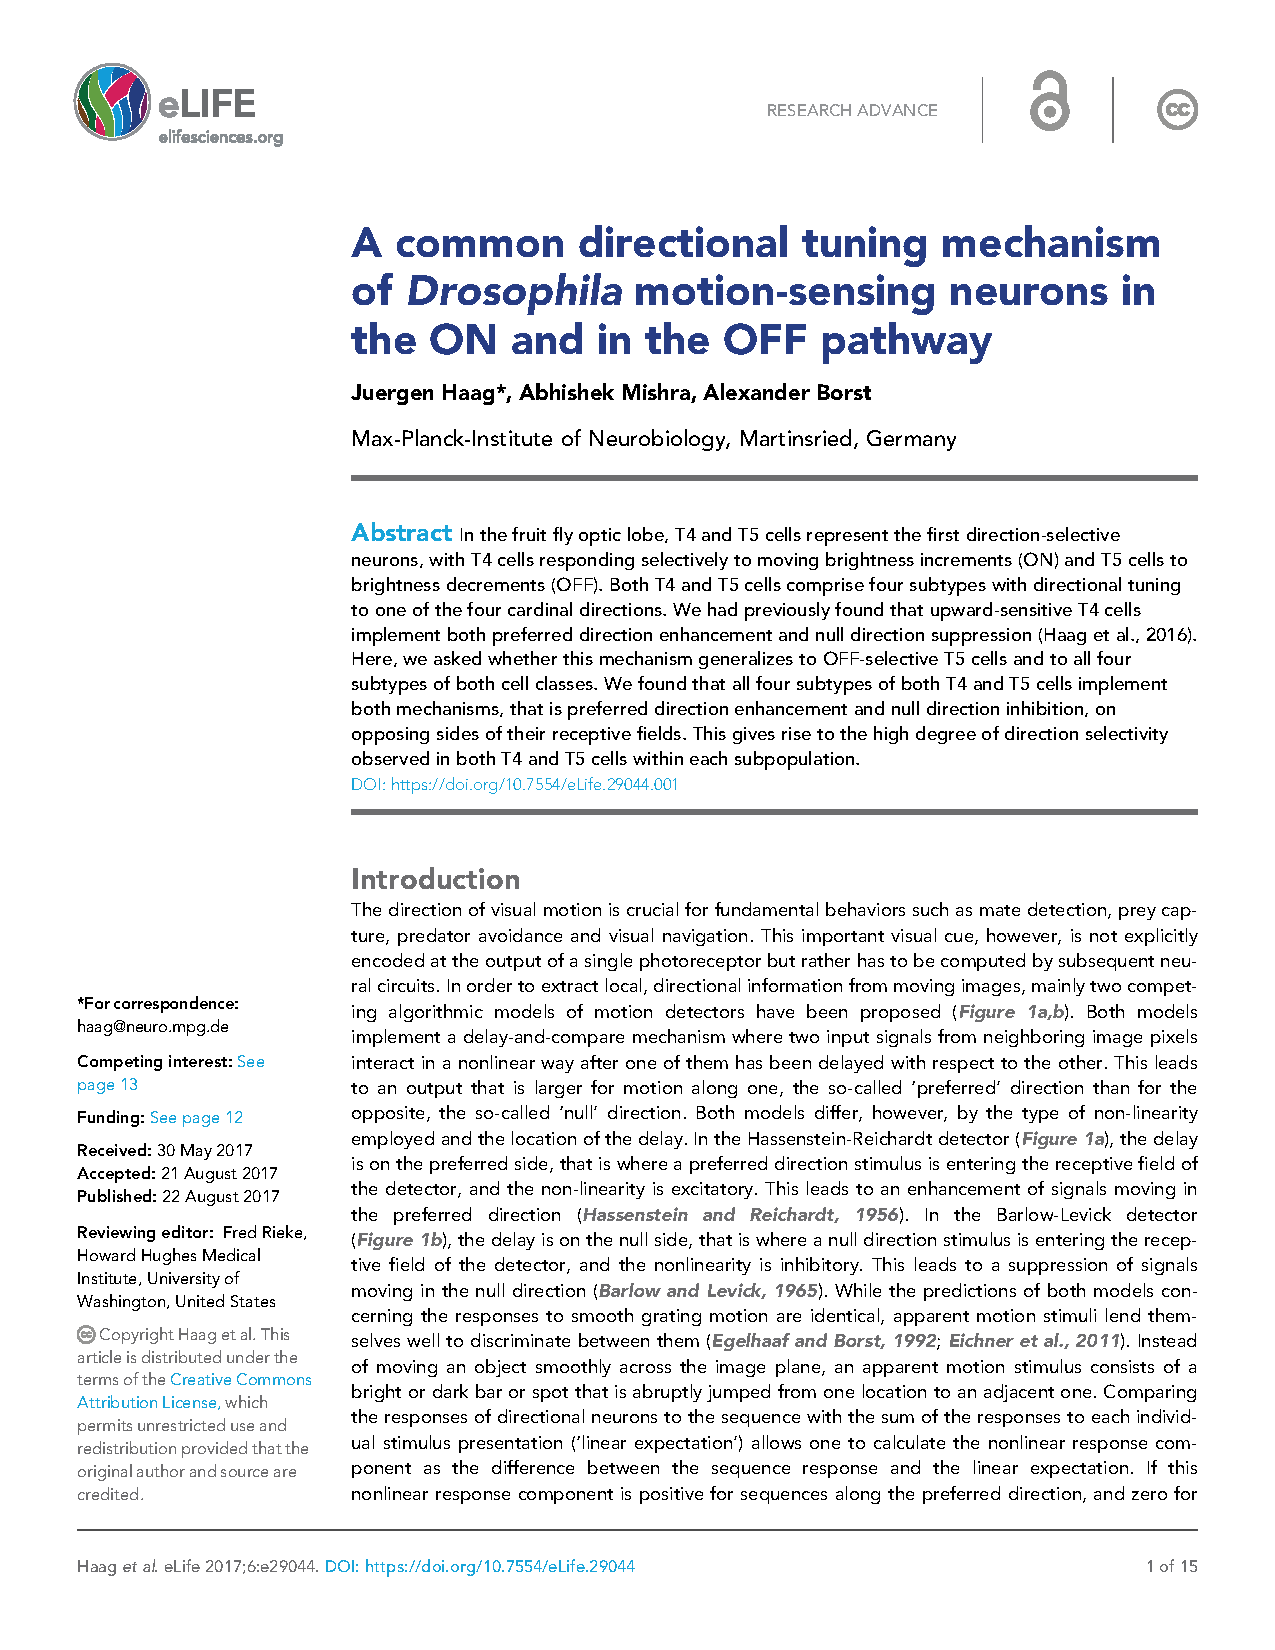
\includepdf[pages=-,scale=0.9,offset= 0 40,pagecommand={\thispagestyle{plain}}]{papers/Haag_Mishra_2017}